\documentclass[11pt]{article} % use larger type; default would be 10pt

\usepackage{tikz}
\usetikzlibrary{calc}
\usetikzlibrary{arrows}
\usetikzlibrary{patterns}
        \newcommand\degree[0]{^{\circ}}

\title{Play with TikZ}
\author{Just Us}
%\date{} % Activate to display a given date or no date (if empty),
         % otherwise the current date is printed 

\begin{document}
\maketitle

\section{Chap 3 Laws of Sines and Cosines}

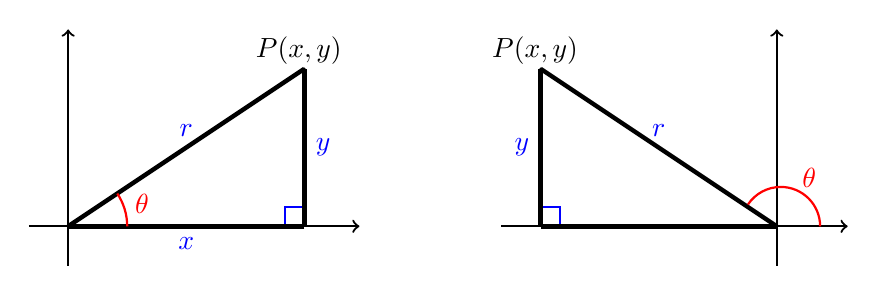
\begin{tikzpicture} 

\coordinate(A) at (3,0);
\coordinate (B) at (3,2);
\coordinate (C) at (0,0);

\filldraw[black] (B) circle (.2pt) node[anchor=south, xshift=-2, yshift=-2] {$P(x,y)$};
\draw[blue,thick] (A) rectangle +(-0.25,0.25);

\draw[black,ultra thick] (A)--(B) node [right,midway] {\color{blue}$y$};
\draw[black,ultra thick] (C)--(B) node [above,midway] {\color{blue}$r$};
\draw[black,ultra thick] (A)--(C) node [below,midway] {\color{blue}$x$};

\draw[black,thick,->] (A) -- ++(0.7,0);
\draw[black,thick] (-.5,0) -- (C);
\draw[black,thick,->] (C)++(0,-0.5) -- +(0,3) ;

\draw[red,thick] (0.75,0) arc (0:{atan(2/3)}:0.75) node[ right, midway, yshift=2] {$\theta$};


% shift
\coordinate(A) at (6,0);
\coordinate (B) at (6,2);
\coordinate (C) at (9,0);

\filldraw[black] (B) circle (.2pt) node[anchor=south, xshift=-2, yshift=-2] {$P(x,y)$};
\draw[blue,thick] (A) rectangle +(0.25,0.25);

\draw[black,ultra thick] (A)--(B) node [left,midway] {\color{blue}$y$};
\draw[black,ultra thick] (C)--(B) node [above,midway] {\color{blue}$r$};
\draw[black,ultra thick] (A)--(C);

\draw[black,thick,->] (C) -- ++(0.9,0);
\draw[black,thick] (A) -- ++(-.5,0);
\draw[black,thick,->] (C)++(0,-0.5) -- +(0,3) ;

\draw[red,thick] (C)++(0.55,0) arc (0:{180-atan(2/3)}:0.5) node[ right, midway, yshift=4] {$\theta$};

\end{tikzpicture}
\newline


fig-3-1-simtri

        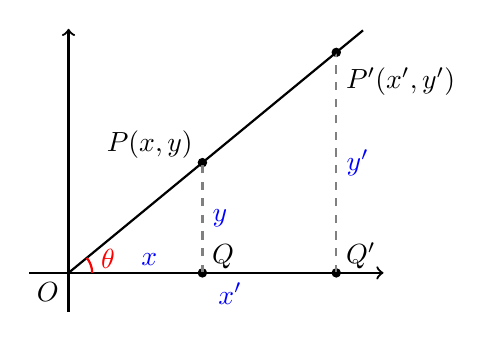
\begin{tikzpicture} 

        \coordinate(A) at (1.7,0);
        \coordinate (B) at (1.7,1.4);
        \coordinate(Ap) at (3.4,0);
        \coordinate (Bp) at (3.4,2.8);
        \coordinate (O) at (0,0);

        \filldraw[black] (O) circle (.2pt) node[anchor=north east, yshift=0] {$O$};
        \filldraw[black] (B) circle (1.5pt) node[anchor=south east, yshift=-2] {$P(x,y)$};
        \filldraw[black] (Bp) circle (1.5pt) node[anchor=north west, yshift=-2] {$P'(x',y')$};
        \filldraw[black] (A) circle (1.5pt) node[anchor=south west, yshift=-2] {$Q$};
        \filldraw[black] (Ap) circle (1.5pt) node[anchor=south west, yshift=-2] {$Q'$};

        \draw[gray,thick, dashed] (A)--(B) node [right,midway] {\color{blue}$y$};
        \draw[gray,thick, dashed] (Ap)--(Bp) node [right,midway] {\color{blue}$y'$};
        \draw[black,thick] (O)--++(3.4,2.8)--++(.34,.28);
        \draw[gray,thick,dashed] (A)--(O) node [above,midway, xshift=5, yshift=-1] {\color{blue}$x$};
        \draw[gray,thick,dashed] (Ap)--(O) node [below,midway, xshift=10] {\color{blue}$x'$};

        \draw[black,thick,->] (-.5,0) -- (4,0);
        \draw[black,thick] (-.5,0) -- (O);
        \draw[black,thick,->] (0,-0.5) -- (0,3.1) ;

        \draw[red,thick] (0.3,0) arc (0:{atan(2.8/3.4)}:0.3) node[ right, midway, yshift=2] {$\theta$};
        \end{tikzpicture}
        \newline


hp3-1-57
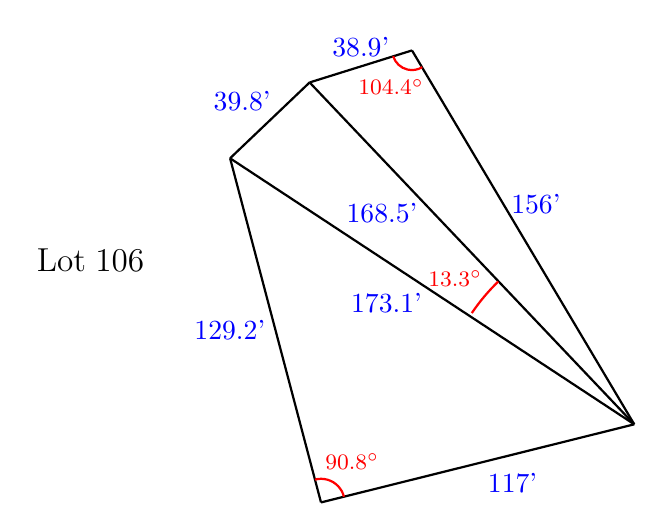
\begin{tikzpicture} [rotate=14]
\coordinate(O) at (0,0);
\coordinate (A) at (4.1,0);
\coordinate (B) at (-.063,4.52);
\coordinate (C) at(1.15,5.21);
\coordinate (D) at (2.51,5.29);

\draw[black,  thick] (O)--(A) node[below right,midway, yshift=0] {\color{blue}117'};
\draw[black,  thick] (O)--(B) node[left,midway, yshift=0] {\color{blue}129.2'};
\draw[black,  thick] (C)--(B) node[above left,midway, xshift=4] {\color{blue}39.8'};
\draw[black,  thick] (C)--(D) node[above,midway, yshift=0] {\color{blue}38.9'};
\draw[black,  thick] (A)--(D) node[above right,midway, xshift=-8, yshift=5] {\color{blue}156'};
\draw[black,  thick] (A)--(B) node[below left,midway, yshift=3] {\color{blue}173.1'};
\draw[black,  thick] (A)--(C) node[below left,midway, xshift=-16, yshift=22] {\color{blue}168.5'};

\draw[red,thick] (O)++(.3,0) arc(0:90.8:.3) node[above right] {\footnotesize$90.8\degree$};
\draw[red,thick] (A)++(-1.66,1.87) arc(132.:120.:2.5) node[above left, midway, xshift=3] {\footnotesize$13.3\degree$};
\draw[red,thick] (D)++(-.25,-.013) arc(183.15:287.45:.25) node[below, midway, xshift=-5] {\footnotesize$104.4\degree$};

\node[text width=3cm] at (-1.3,3.5) 
    {\large Lot 106};
\end{tikzpicture}
\newline

hp3-1-58
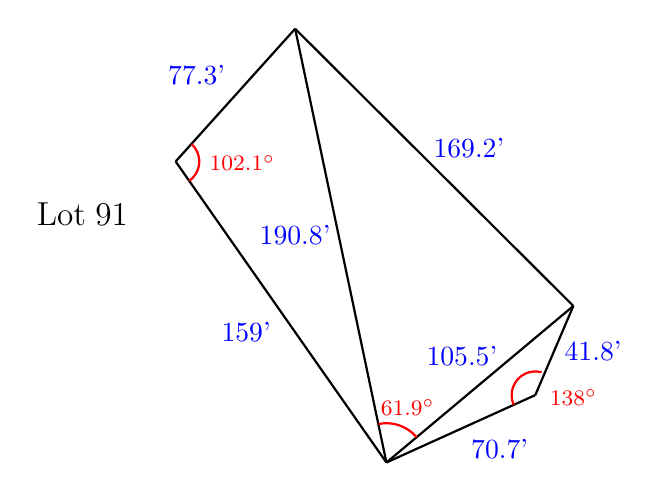
\begin{tikzpicture} [rotate=-55]
\coordinate(O) at (0,0);
\coordinate (A) at (4.667,0);
\coordinate (B) at (-.51,2.21);
\coordinate (C) at(4.4,3.085);
\coordinate (D) at (5.05,2.04);

\draw[black, thick] (O)--(A) node[below left,midway, yshift=0] {\color{blue}159'};
\draw[black,  thick] (O)--(B) node[above left,midway, yshift=0] {\color{blue}77.3'};
\draw[black,  thick] (C)--(B) node[above right,midway, xshift=-4] {\color{blue}169.2'};
\draw[black,  thick] (C)--(D) node[right,midway, yshift=0] {\color{blue}41.8'};
\draw[black,  thick] (A)--(D) node[below right,midway, xshift=0, yshift=0] {\color{blue}70.7'};
\draw[black,  thick] (A)--(B) node[left,midway, yshift=4] {\color{blue}190.8'};
\draw[black,  thick] (A)--(C) node[above left,midway, xshift=10, yshift=3] {\color{blue}105.5'};

\draw[red,thick] (O)++(.3,0) arc(0:102.1:.3) node[right,midway] {\footnotesize$102.1\degree$};
\draw[red,thick] (A)++(-.459,.197) arc(156.8:94.9:.5) node[above, midway, xshift=3] {\footnotesize$61.9\degree$};
\draw[red,thick] (D)++(-.055,-.295) arc(-100.5:-230.5:.3) node[below right, midway, xshift=8] {\footnotesize$138\degree$};

\node[text width=3cm] at (.4,-.6) {\large Lot 91};
\end{tikzpicture}
\newline


hp3-1-7
        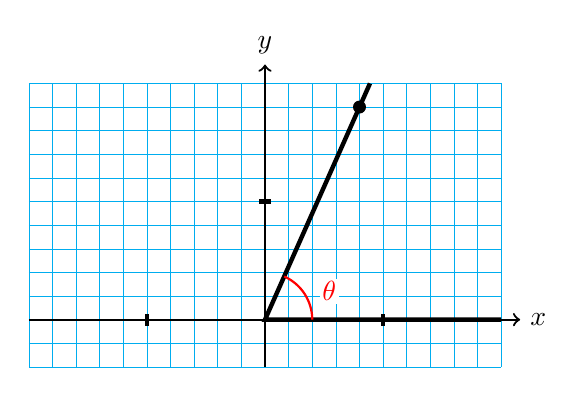
\begin{tikzpicture}[scale=.3]

        \draw[step=1cm,cyan,very thin] (-10,-2) grid (10,10);
        \draw[thick,->] (-10,0) -- (10.8,0) node[anchor=west] {$x$};
        \draw[thick,->] (0,-2) -- (0,10.8) node[anchor=south] {$y$};
        \draw[ultra thick] (-5,0)+(0,-.25) -- +(0,.25);
        \draw[ultra thick] (5,0)+(0,-.25) -- +(0,.25);
        \draw[ultra thick] (0,5)+(-.25,0) -- +(.25,0);

        \coordinate (O) at (0,0);

        \coordinate (P) at (4,9);

        \filldraw[black] (P) circle (.25cm) ;

        \draw[black, ultra thick] (10,0)--(O)--(P)--+(.444,1) ;
        \draw[red, thick] (O)++(2cm,0) arc(0:{atan(9/4)}:2cm) node[right,midway, xshift=5, yshift=1,fill=white,inner sep=1pt] {$\theta$};
\end{tikzpicture}
\newline



act3-1
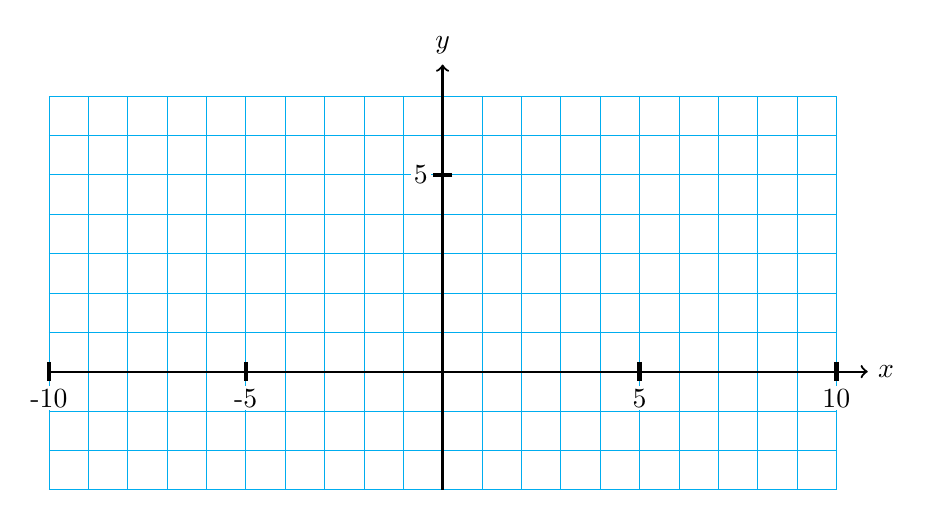
\begin{tikzpicture}[scale=.5]

\draw[step=1cm,cyan,very thin] (-10,-3) grid (10,7);
\draw[thick,->] (-10,0) -- (10.8,0) node[anchor=west] {$x$};
\draw[thick,->] (0,-3) -- (0,7.8) node[anchor=south] {$y$};
\foreach \x in {-10, -5,5,10}
    \draw[ultra thick] (\x cm,0)+(0,.25) -- +(0,-.25) node[below, yshift=-1,fill=white, inner sep=1pt] {\x};

    \draw[ultra thick] (0,5 cm)+(.25,0) -- +(-.25,0) node[left,fill=white, inner sep=1pt] {5};
\end{tikzpicture}
\newline

exam3-2-5

    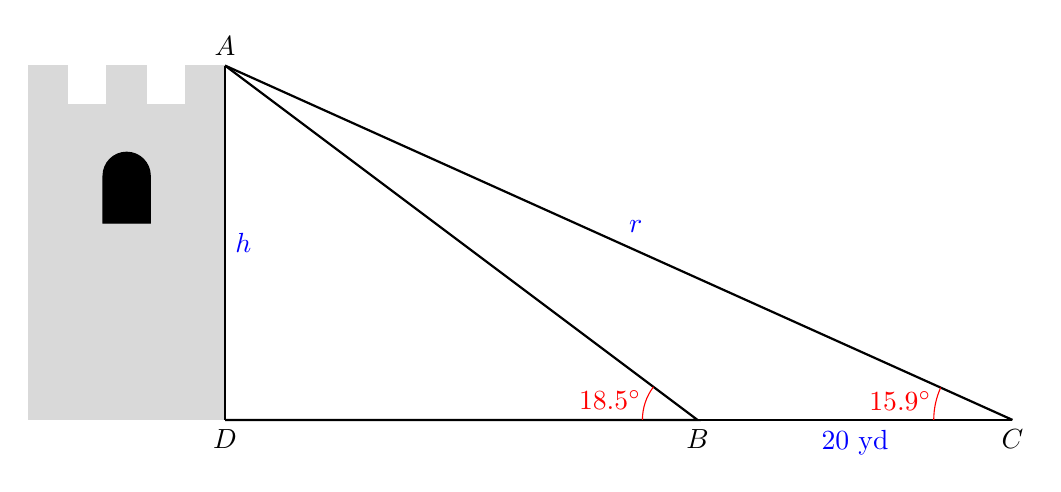
\begin{tikzpicture} 

    \filldraw[gray!30!white] (0,0) -- ++(0,4.5) -- ++(-.5,0) -- ++(0,-.5) -- ++(-.5,0) -- ++(0,.5) -- ++(-.5,0) -- ++(0,-.5) -- ++(-.5,0) -- ++(0,.5) -- ++(-.5,0) -- ++(0,-4.5)--cycle;

    \filldraw[black] (-1.55,2.5) -- ++(.6,0) -- ++(0,.6) arc(0:180:.3) -- cycle;

    \coordinate (D) at (0,0);
    \coordinate (A) at (0,4.5);
    \coordinate (B) at (6,0);
    \coordinate (C) at (10,0);

    \draw[black] (A) node[anchor=south] {$A$};
    \draw[black] (B) node[anchor=north] {$B$};
    \draw[black] (C) node[anchor=north] {$C$};
    \draw[black] (D) node[anchor=north] {$D$};

    \draw[black, thick] (C)--(B) node[below,midway] {\color{blue}20 yd};
    \draw[black, thick] (A)--(B)--(D);
    \draw[black, thick] (A)--(C) node[above right,midway] {\color{blue}$r$};
    \draw[black, thick] (A)--(D) node[right,midway] {\color{blue}$h$};
    
    \draw[red] (B)++(-.7,0) arc(180:{180-atan(3/4)}:.7) node[left, xshift=2, yshift=1, midway]{$18.5\degree$};
    \draw[red] (C)++(-1,0) arc(180:{180-atan(9/20)}:1) node[left, xshift=2, yshift=1, midway]{$15.9\degree$};
        \end{tikzpicture}



exam4-1-1

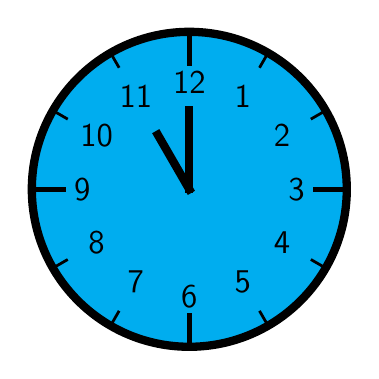
\begin{tikzpicture}[line cap=rect,line width=3pt]
\filldraw [fill=cyan] (0,0) circle [radius=2cm];
\foreach \angle [count=\xi] in {60,30,...,-270}
{
  \draw[line width=1pt] (\angle:1.8cm) -- (\angle:2cm);
  \node[font=\large] at (\angle:1.36cm) {\textsf{\xi}};
}
\foreach \angle in {0,90,180,270}
  \draw[line width=2pt] (\angle:1.6cm) -- (\angle:2cm);
\draw (0,0) -- (120:0.8cm);
\draw (0,0) -- (90:1cm);
\end{tikzpicture}
\newline


hp3-2-33 30-60-90 triangle
\begin{tikzpicture} 
\coordinate (A) at (0,0);
\coordinate (B) at (30:3);
\coordinate (C) at($ 3*cos(30)*(1,0) $);
\coordinate (D) at (4,0);

\filldraw[black] (A) circle (.5pt) node[anchor = north east] {$A$};
\filldraw[black] (B) circle (.5pt) node[anchor = south] {$B$};
\filldraw[black] (C) circle (.5pt) node[anchor = north] {$C$};
\draw[blue, thick] (C) rectangle +(-.25, .25);

\draw[black, thick] (B)--(A) node[above left,midway, yshift=0] {\color{blue} 3};
\draw[black,  thick] (C)--(B) node[right,midway, yshift=0] {\color{blue}$a$};
\draw[black,  thick] (D)--(A) ;

\draw[red,thick] (O)++(.5,0) arc(0:30:.5) node[right,midway, yshift=2] {\footnotesize$30\degree$};

\end{tikzpicture}
\newline


hp3-sum-41ans

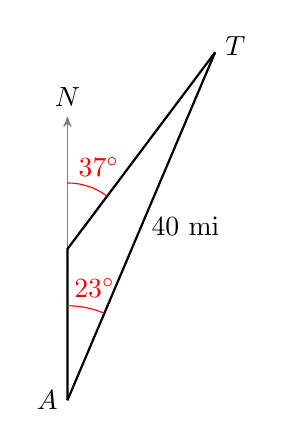
\begin{tikzpicture} [scale=1.2]
\coordinate(A) at (0,0);
\coordinate(N) at (0,3);
\coordinate(T) at (67:4);
\coordinate(x) at (0,1.6);
\draw[gray,->,>=stealth'] (A)--(N) node[above, text=black]{$N$};
\draw[black,thick] (A)--(x)--(T) node[above right, yshift=-5]{$T$};
\draw[black,thick] (A)--(T) node[right, midway]{40 mi};
\draw[red] (0,1) arc(90:67:1) node[above, midway, xshift=3] {$23\degree$};
\draw[red] (0,2.3) arc(90:54:0.7) node[above, midway, xshift=4] {$37\degree$};
\node[left] at (A) {$A$};
\end{tikzpicture}
\newline





\section {Stuff for later}


part A: law of sines a circumscribing circle

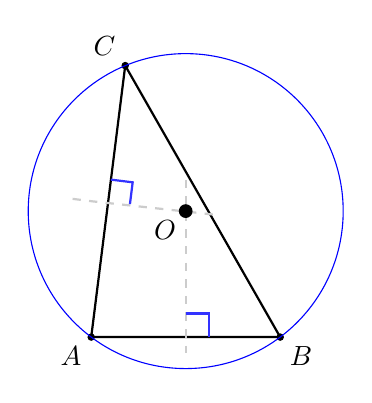
\begin{tikzpicture} [scale=.4]

\coordinate (O) at (0,0);
\coordinate (A) at (-3,-4);
\coordinate (B) at (3,-4);
\coordinate (C) at (-1.92,4.62);

\filldraw (A) circle (.1cm) node[anchor=north east] {$A$};
\filldraw (B) circle (.1cm) node[anchor=north west] {$B$};
\filldraw (C) circle (.1cm) node[anchor=south east] {$C$};

\draw[black,thick] (A)--(B)--(C)--(A);
\draw[gray!40!white, thick, dashed](O)++(0,1) -- (0,-4)--+(0,-.5);
\draw[gray!40!white, thick, dashed](O)++(.862,-.108) -- (-2.96,.31)--++(-.862,.108);
\draw[blue!80!white,thick] (0,-4)++(.75,0)-- ++(0,.75) -- ++(-.75,0);
\draw[blue!80!white,thick] (-2.46,.31) ++(.0864,.6896) -- ++(.6896,-.0864) -- ++(-.0864,-.6896);
\filldraw (O) circle (.2cm) node[anchor=north east] {$O$};

\draw[blue] (O) circle (5);

\end{tikzpicture}
\newline

part B: law of sines a circumscribing circle

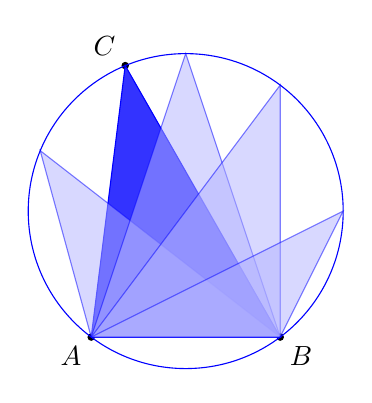
\begin{tikzpicture} [scale=.4]

\coordinate (O) at (0,0);
\coordinate (A) at (-3,-4);
\coordinate (B) at (3,-4);
\coordinate (C) at (-1.92,4.62);
\coordinate (Cp) at (-4.62,1.92);
\coordinate (Cpp) at (0,5);
\coordinate (Cppp) at (3,4);
\coordinate (Cpppp) at (5,0);

\filldraw (O) circle (.1cm) node[anchor=north east] {$O$};
\filldraw (A) circle (.1cm) node[anchor=north east] {$A$};
\filldraw (B) circle (.1cm) node[anchor=north west] {$B$};
\filldraw (C) circle (.1cm) node[anchor=south east] {$C$};

\draw[draw= blue, fill=blue!80!white] (A)--(B)--(C)--(A);
\draw[draw= blue, fill=blue!30!white, opacity=.5] (A)--(B)--(Cp)--(A);
\draw[draw= blue, fill=blue!30!white, opacity=.5] (A)--(B)--(Cpp)--(A);
\draw[draw= blue, fill=blue!30!white, opacity=.5] (A)--(B)--(Cppp)--(A);
\draw[draw= blue, fill=blue!30!white, opacity=.5] (A)--(B)--(Cpppp)--(A);


\draw[blue] (O) circle (5);

\end{tikzpicture}
\newline


Section 4.2 Angle of inclination
\begin{tikzpicture}

\coordinate (O) at (0,0);
\coordinate (x) at (3.5,0);
\coordinate (y) at (0,2);
\coordinate (A) at (3,1.8);
\coordinate (B) at (1.,0);
\coordinate (C) at (2.5,0);
\coordinate (D) at (-1,-1.8);

\draw[black,  thick, ->] (-1.5,0) --  (x) node[right] {$x$} ;
\draw[black,  thick, ->] (0,-2) --  (y) node[above] {$y$}  ;
\draw[black,  thick, <->] (D) --  (A)  ;
\draw[red, thick] (1.9,0) arc (0:{atan(0.9)}:.9) node [left, midway,xshift=0,yshift=-3] {$\alpha$};

\end{tikzpicture}
\newline

Section 4.2 Angle of inclination
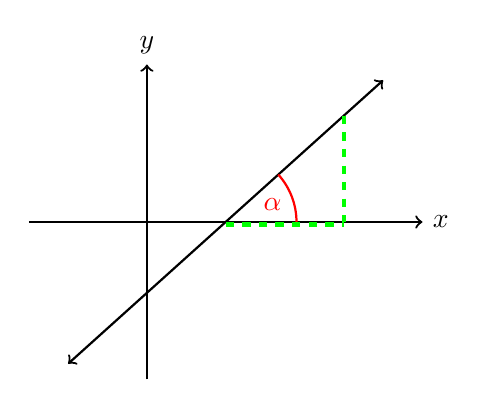
\begin{tikzpicture}

\coordinate (O) at (0,0);
\coordinate (x) at (3.5,0);
\coordinate (y) at (0,2);
\coordinate (A) at (3,1.8);
\coordinate (B) at (1.,0);
\coordinate (C) at (2.5,0);
\coordinate (D) at (-1,-1.8);

\draw[black,  thick, ->] (-1.5,0) --  (x) node[right] {$x$} ;
\draw[black,  thick, ->] (0,-2) --  (y) node[above] {$y$}  ;
\draw[black,  thick, <->] (D) --  (A)  ;
\draw[red, thick] (1.9,0) arc (0:{atan(0.9)}:.9) node [left, midway,xshift=0,yshift=-3] {$\alpha$};

\draw[green, ultra thick, dashed] (1,-.03) -- (2.5,-.03);
\draw[green, ultra thick, dashed] (2.5,1.35) -- (2.5,0);

\end{tikzpicture}
\newline


On a unit circle
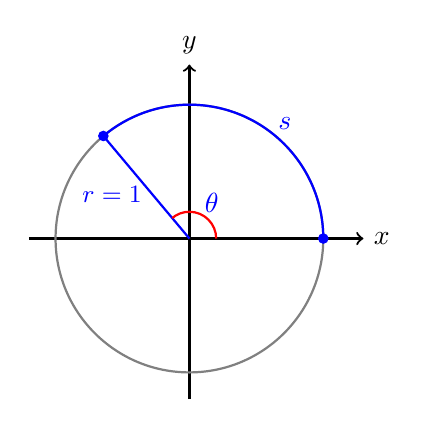
\begin{tikzpicture} [scale=1.7]

\draw[thick,->] (-1.2,0) -- (1.3,0) node[anchor=west] {$x$};
\draw[thick,->] (0,-1.2) -- (0,1.3) node[anchor=south] {$y$};

\coordinate(O) at (0,0);
\coordinate(A) at (1,0);
\coordinate (B) at (-.6428,0.766);

\draw[gray,thick] (O) circle (1);
\draw[blue,thick] (O) -- (B) node[below left, midway, xshift=2, yshift=4] {\small\color{blue} $r=1$};
\filldraw [blue] (A) circle (1pt);
\filldraw [blue] (B) circle (1pt);
\draw[blue,thick] (A) arc(0:130:1) node[above, midway, xshift=14, yshift=-8] {\color{blue}$s$};
\draw[red,thick] (O)++(.2,0) arc(0:130:.2) node[above, midway, xshift=4, yshift=-3] {\color{blue}$\theta$};

\end{tikzpicture}
\newline


Exercise not used?
\begin{tikzpicture}
\coordinate (O) at (0,0);
\coordinate (A) at (0,0);
\coordinate (B) at (0,0);
\coordinate(C) at (0,0);
\coordinate (D) at (0,0);
\filldraw[black] (O) circle (.2pt) node[anchor=south west, xshift=6]{$50\degree$};
\filldraw[black] (A) circle (.2pt) node[anchor=south east]{$x$};
\filldraw[black] (B) circle (.2pt) node[anchor=north east, xshift=-6]{$y$};
\filldraw[black] (C) circle (.2pt) node[anchor=north west]{$z$};
%\draw[black,  thick] (A) -- (B) --( C) -- cycle;
\draw[black] (-2.3,0) --  (2.3,0);
\draw[black] (0.8,1.3) --  (-0.8,-1.3) ;
\end{tikzpicture}
\newline


\end{document}
